
% This LaTeX was auto-generated from MATLAB code.
% To make changes, update the MATLAB code and republish this document.

\documentclass{article}
\usepackage{graphicx}
\usepackage{color}
\pdfminorversion=7

\sloppy
\definecolor{lightgray}{gray}{0.5}
\setlength{\parindent}{0pt}

\begin{document}

    
    
\subsection*{Contents}

\begin{itemize}
\setlength{\itemsep}{-1ex}
   \item Experiment 01: Plot Raw Data vs Time
   \item 01 Questions and Answers
   \item Experiment 02: Plot Raw Data vs Time
   \item Experiment 02: Plot LowPass Filtered Data vs Time
   \item 02 Questions and Answers
\end{itemize}


\subsection*{Experiment 01: Plot Raw Data vs Time}


\color{lightgray} \begin{verbatim}

Chest Lying Down Heart Rate: 72 
Hand Lying Down Heart Rate: 62 


\end{verbatim} \color{black}

The previous heartrates were calculated by using the ismax function and plotting the R wave from the depolarization of the heart beating. This was fine tuned until a reasonable accounting of the heart beat could be used. 

\vspace{2em}
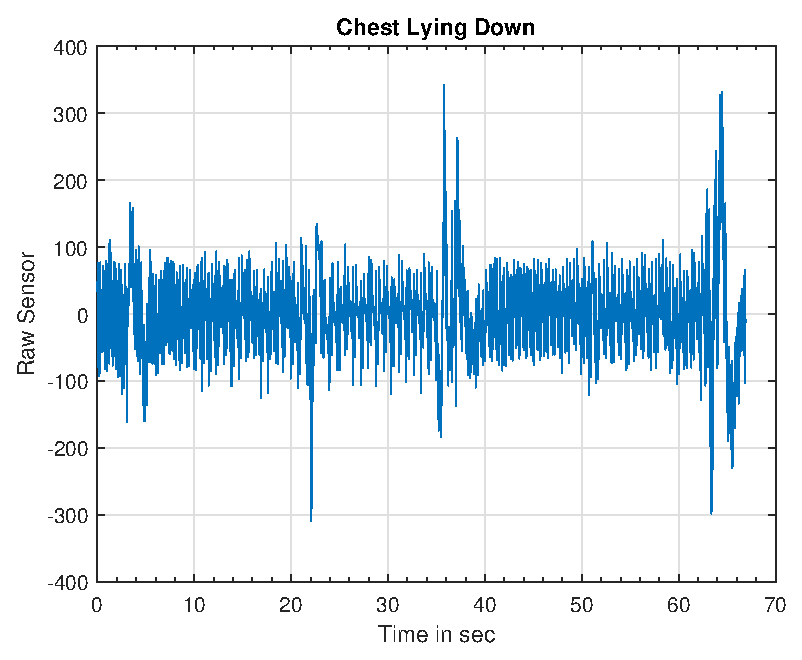
\includegraphics [width=4in]{Lab04_01.eps}

\begin{verbatim} 
ismax = islocalmax(rawData(k).ecg,'MinProminence',35);
maxIndices = find(ismax);
msPerBeat = mean(diff(maxIndices));
heartRate = 60*(100/msPerBeat);
\end{verbatim}

\vspace{2em}
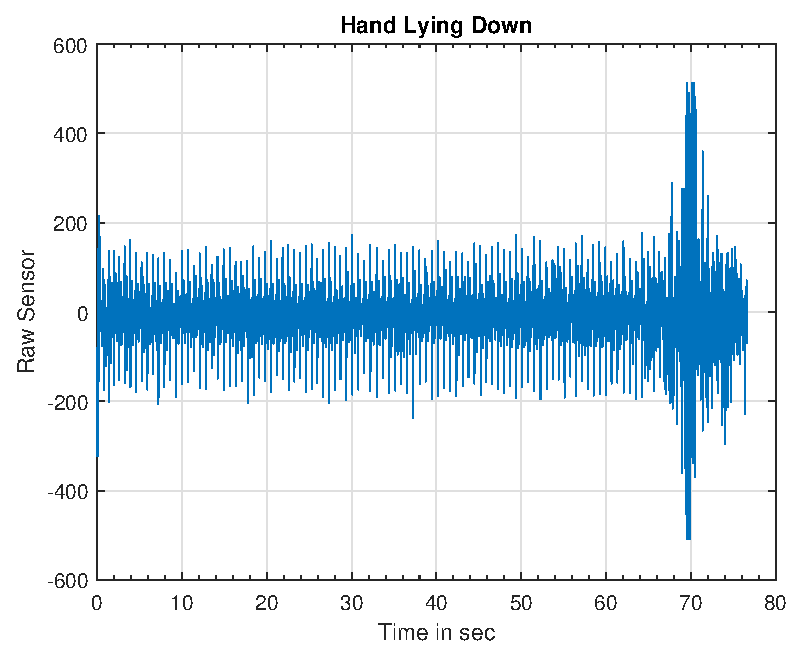
\includegraphics [width=4in]{Lab04_02.eps}

\begin{verbatim} 
ismax = islocalmax(rawData(k).ecg,'MinProminence',65);
maxIndices = find(ismax);
msPerBeat = mean(diff(maxIndices));
heartRate = 60*(100/msPerBeat);
\end{verbatim}

\subsection*{01 Questions and Answers}

\begin{par}
Was there variability between the beats? Would you expect the interval between beats to be identical? Why or why not?

\vspace{1em}
There was variability between the beats. This makes sense as the distance from
the heart was different. I would expect the variability between beats to be
extremely close however. Assuming a healthy blood vessel system, then I
couldn't imagine any issues with the

\end{par} \vspace{1em}


\subsection*{Experiment 02: Plot Raw Data vs Time}


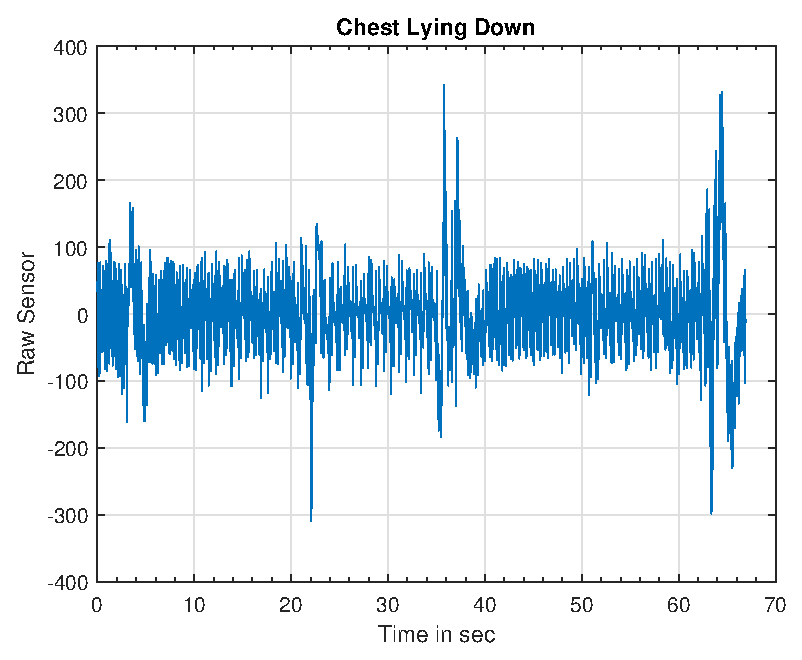
\includegraphics [width=4in]{Lab04_03.eps}
\vspace{2em}
\vspace{1em}
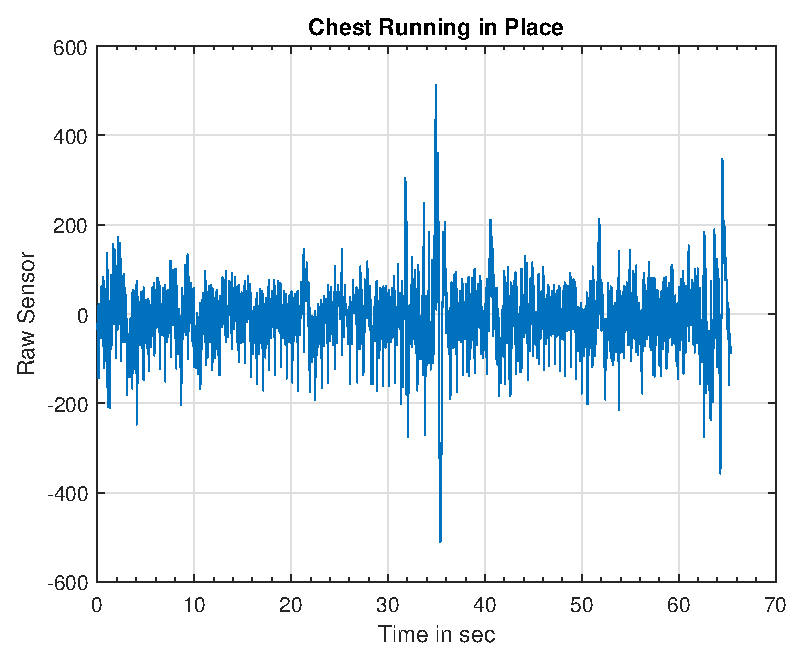
\includegraphics [width=4in]{Lab04_04.eps}
\vspace{2em}
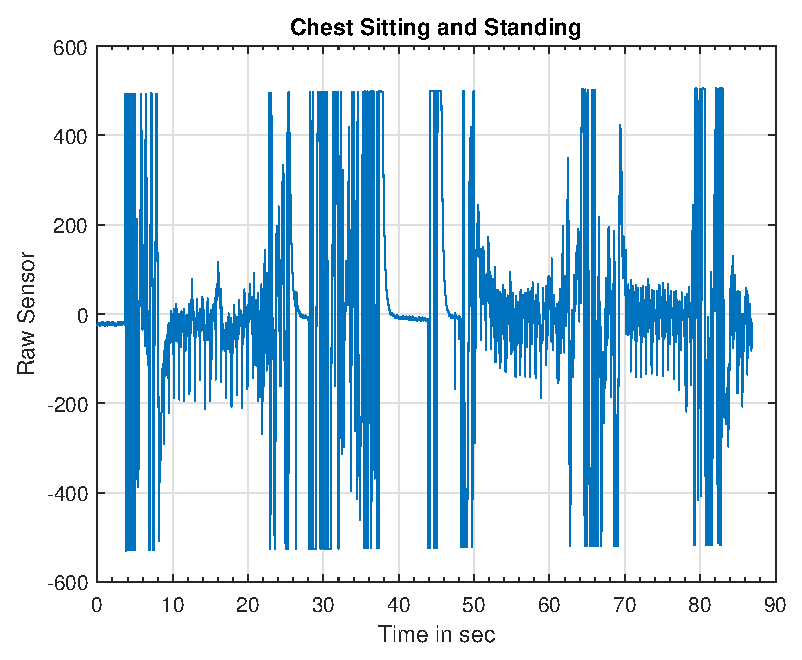
\includegraphics [width=4in]{Lab04_05.eps}
\vspace{2em}
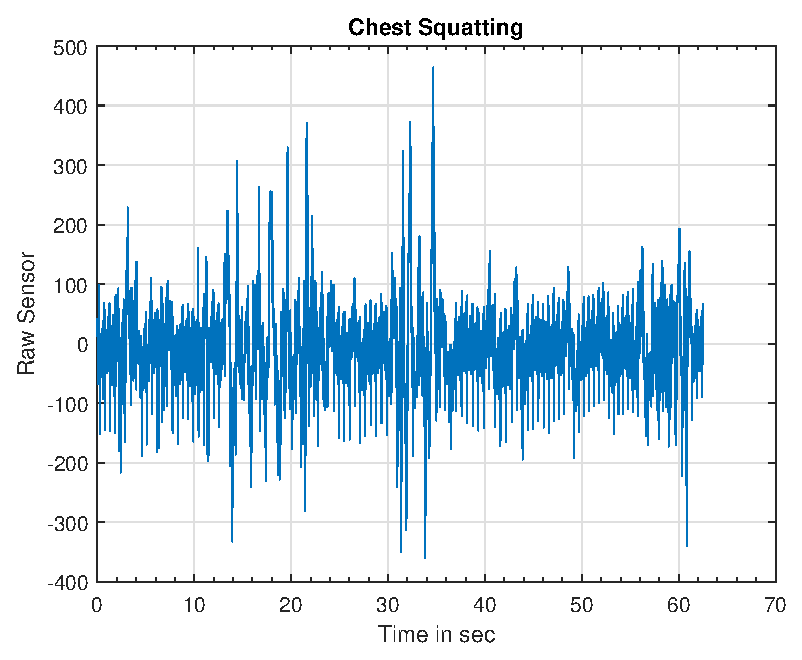
\includegraphics [width=4in]{Lab04_06.eps}
\vspace{2em}
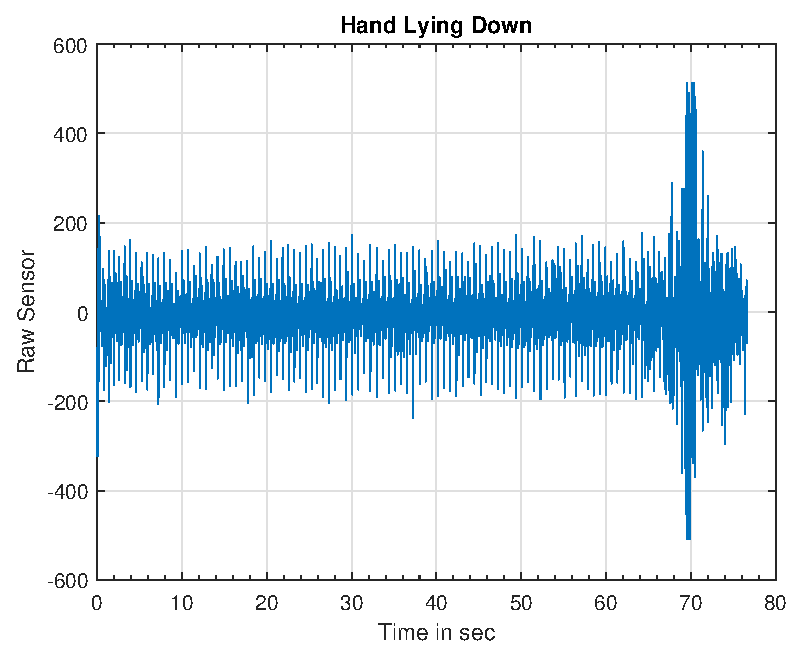
\includegraphics [width=4in]{Lab04_07.eps}
\vspace{2em}
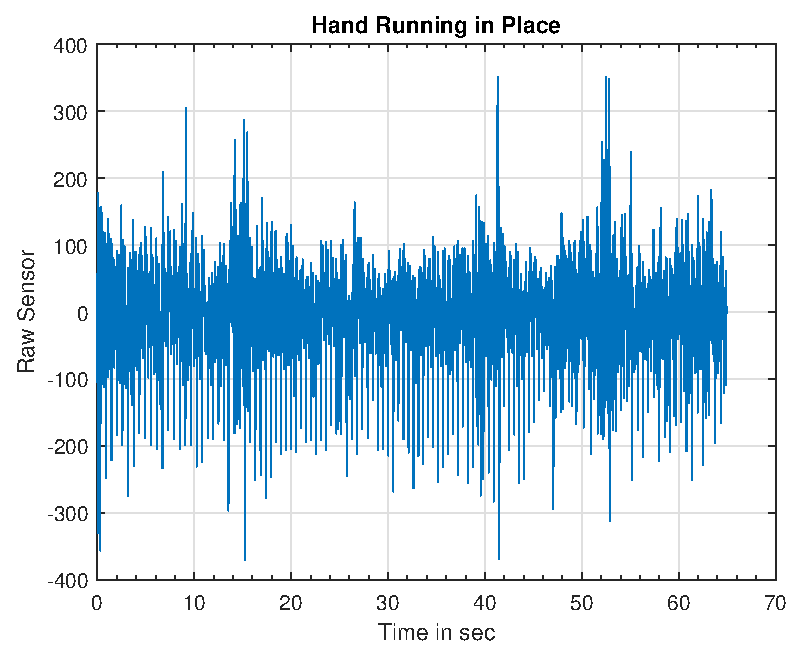
\includegraphics [width=4in]{Lab04_08.eps}
\vspace{2em}
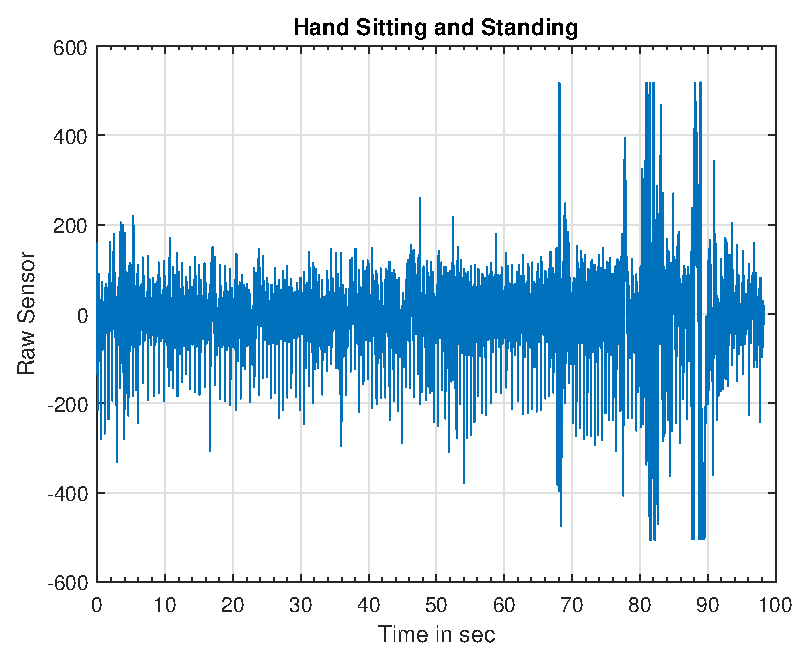
\includegraphics [width=4in]{Lab04_09.eps}
\vspace{2em}
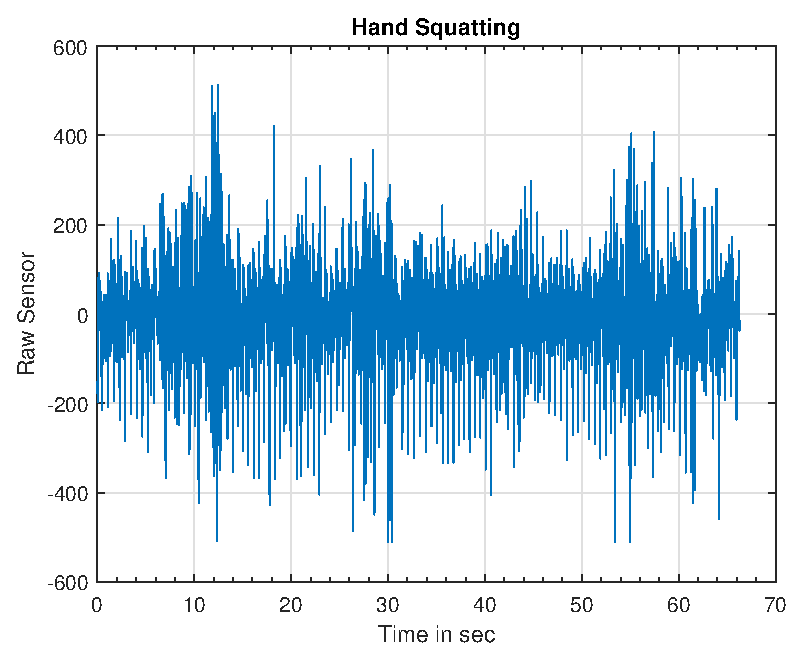
\includegraphics [width=4in]{Lab04_10.eps}


\subsection*{Experiment 02: Plot LowPass Filtered Data vs Time}

\vspace{2em}
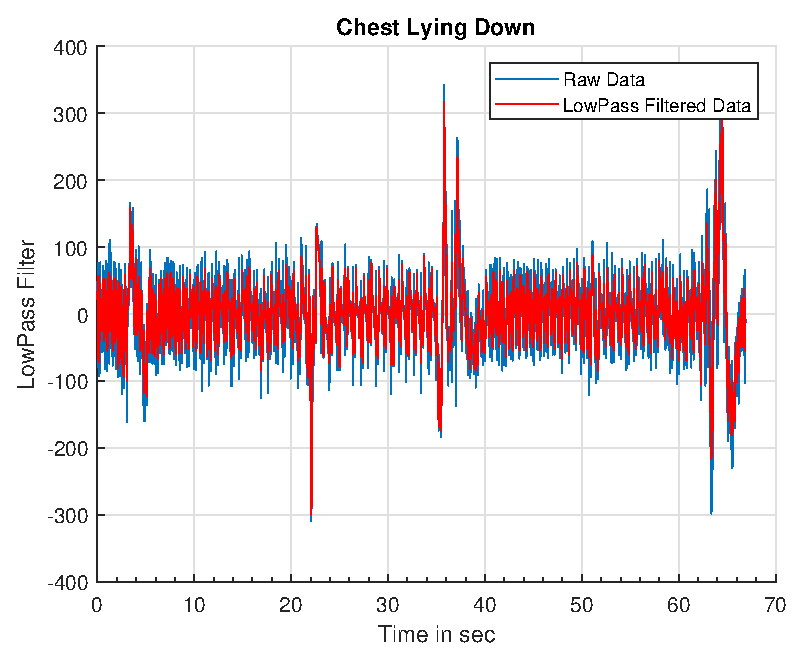
\includegraphics [width=4in]{Lab04_11.eps}
\vspace{2em}
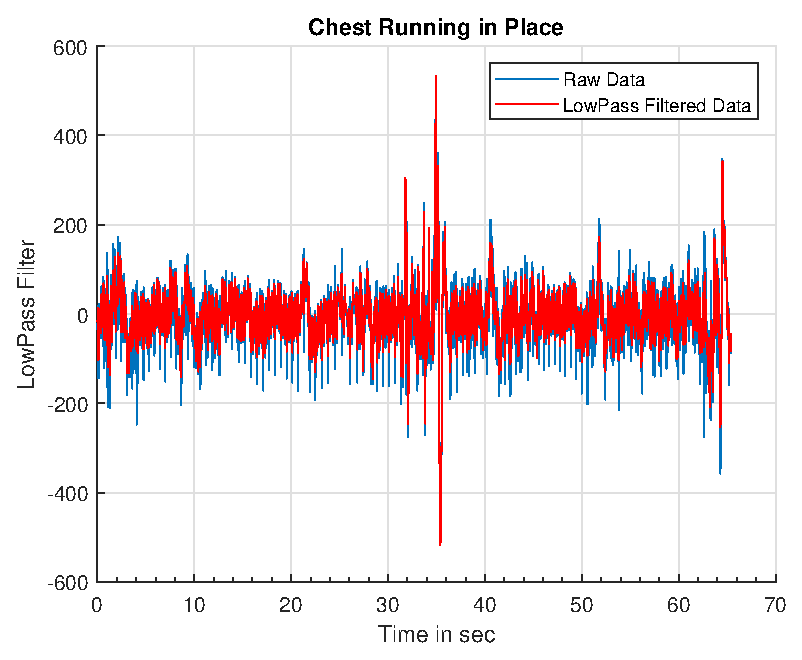
\includegraphics [width=4in]{Lab04_12.eps}
\vspace{2em}
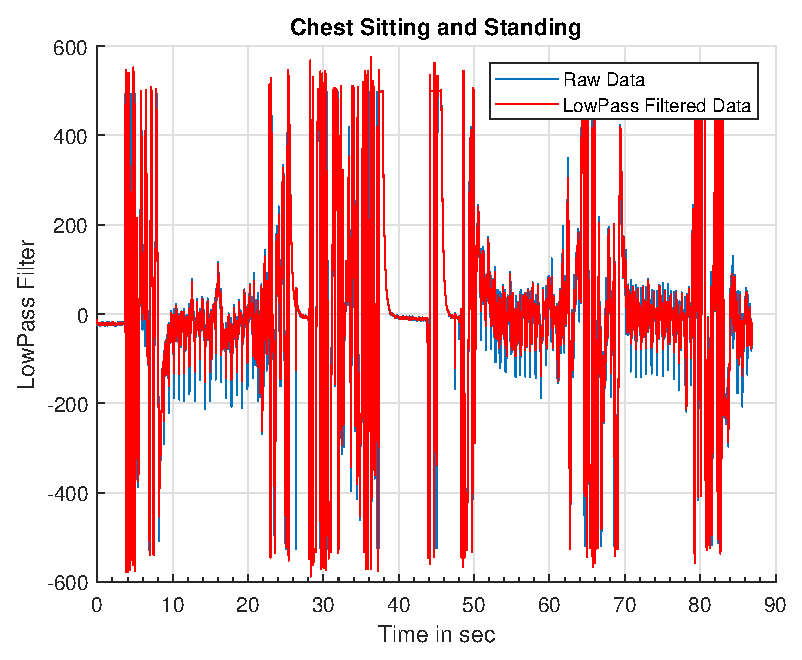
\includegraphics [width=4in]{Lab04_13.eps}
\vspace{2em}
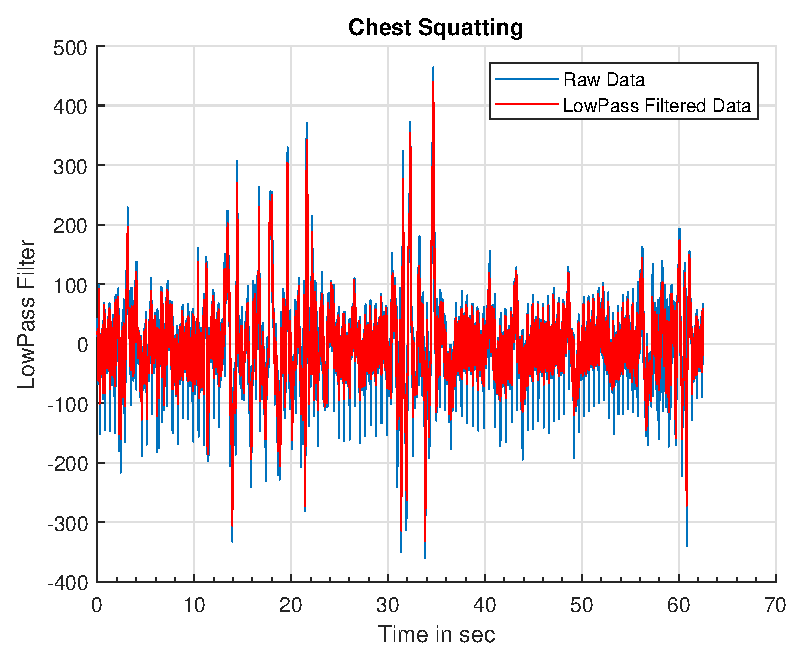
\includegraphics [width=4in]{Lab04_14.eps}
\vspace{2em}
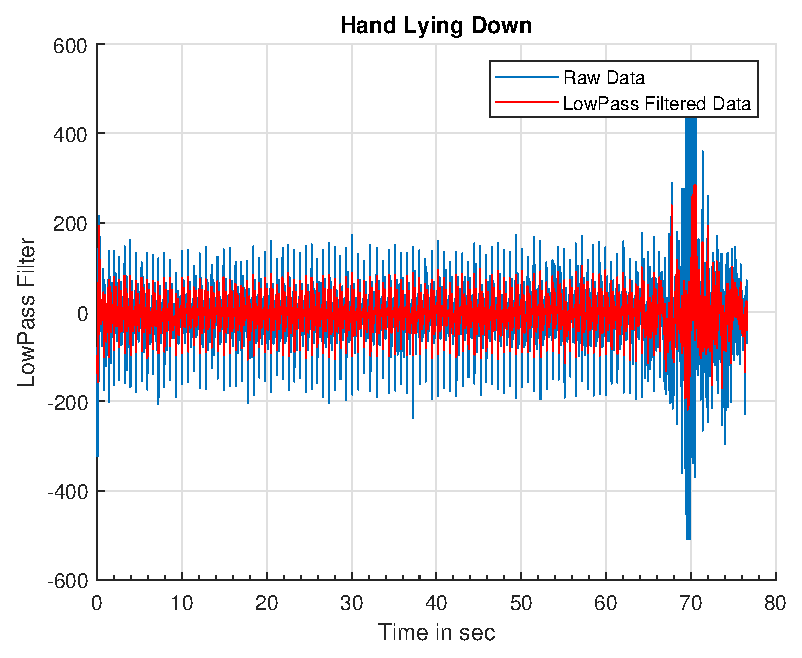
\includegraphics [width=4in]{Lab04_15.eps}
\vspace{2em}
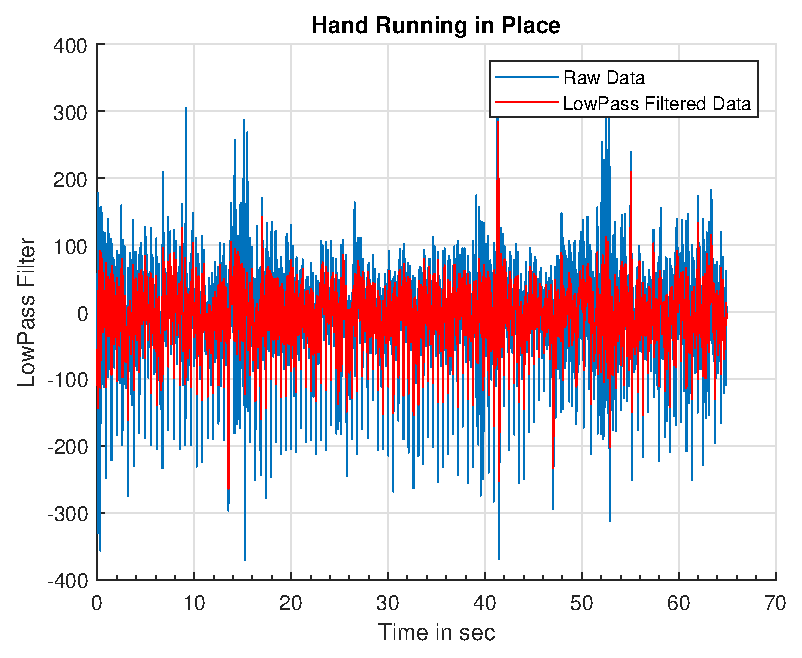
\includegraphics [width=4in]{Lab04_16.eps}
\vspace{2em}
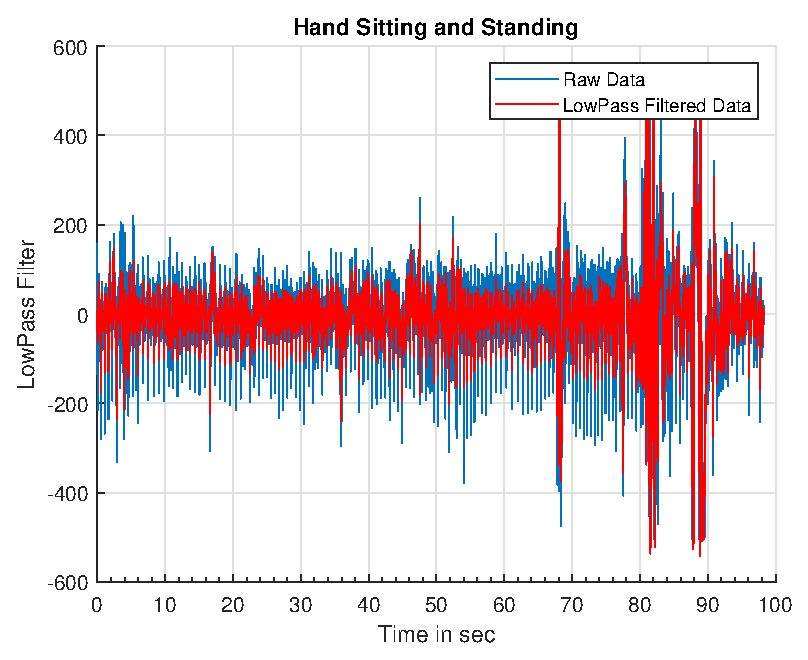
\includegraphics [width=4in]{Lab04_17.eps}
\vspace{2em}
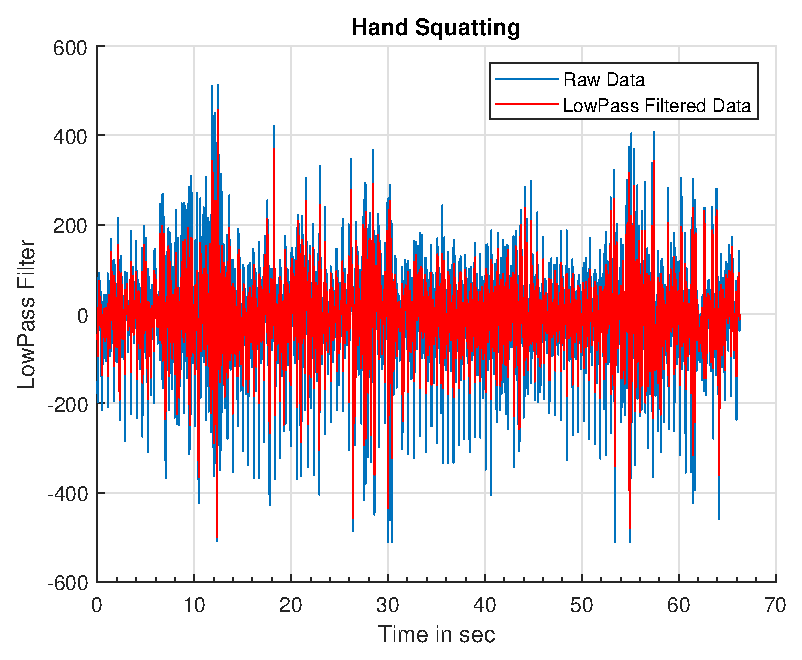
\includegraphics [width=4in]{Lab04_18.eps}


\subsection*{02 Questions and Answers}

\begin{par}
What physiological advantage is there in a slower resting heart rate?

\vspace{1em}
A slower resting heart rate means your heart is more efficient at pumping
oxengentated blood around your body. Since it is stronger, it pumps less
often, causing less wear on the heart over the lifetime of the person. Also it
likely means that the heart can recover from high periods of activity faster,
returning to a lower rate and easing the workload much faster than a not as
healthy heart.
\end{par} \vspace{1em}

\end{document}

